\documentclass[11pt]{article}
\usepackage[utf8]{inputenc}
\usepackage{tikz}
\usetikzlibrary{shapes.geometric, arrows}

\tikzstyle{startstop} =[rectangle, rounded corners, minimum width =3cm, minimum height=1cm ,text centered, draw=black , fill =red!20]
\tikzstyle{io}= [trapezium, trapezium left angle =70 ,trapezium right angle =110, minimum width =3cm, minimum height =1cm,text centered, draw=black, fill= blue!20]
\tikzstyle{process} =[rectangle, minimum width= 3cm , minimum height =1cm , text centered, draw=black, fill = orange!50]
\tikzstyle{decision} =[diamond, minimum width =3cm, minimum height =1cm, text centered, draw=black , fill =green!30]
\tikzstyle{arrow} =[thick,->,>=stealth]
\begin{document}

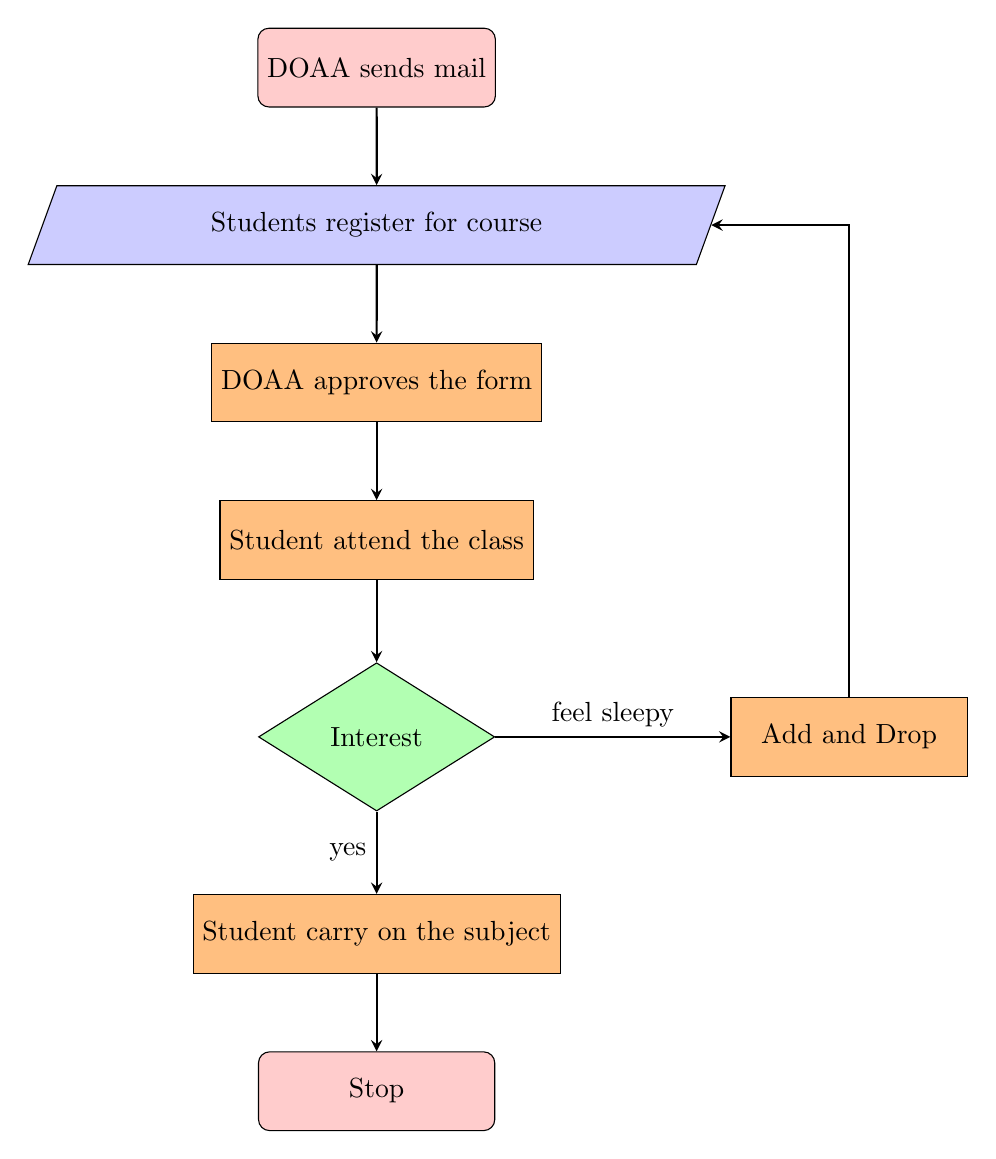
\begin{tikzpicture}[node distance=2cm]
\node (start) [startstop] {DOAA sends mail};
\node (in1) [io,below of=start] {Students register for course};
\node (pro1) [process, below of=in1] {DOAA approves the form};
\node (pro2) [process, below of=pro1] {Student attend the class};
\node (dec1) [decision , below of=pro2 , yshift=-0.5cm] {Interest};
\node (pro3) [process, below of= dec1, yshift= -0.5cm] {Student carry on the subject};
\node (pro4) [process, right of = dec1, xshift= 4cm] {Add and Drop};
\node (stop) [startstop, below of =pro3] {Stop};

\draw [arrow] (start)--(in1);
\draw [arrow] (in1)--(pro1);
\draw [arrow] (pro1)--(pro2);
\draw [arrow] (pro2)--(dec1);
\draw [arrow] (dec1)--node[anchor=east]{yes}(pro3);
\draw [arrow] (dec1)--node[anchor=south]{feel sleepy}(pro4);
\draw [arrow] (pro4)|-(in1);
\draw [arrow] (pro3)--(stop);
\end{tikzpicture}
\end{document}


